\chapter{Příloha}

\begin{figure}
	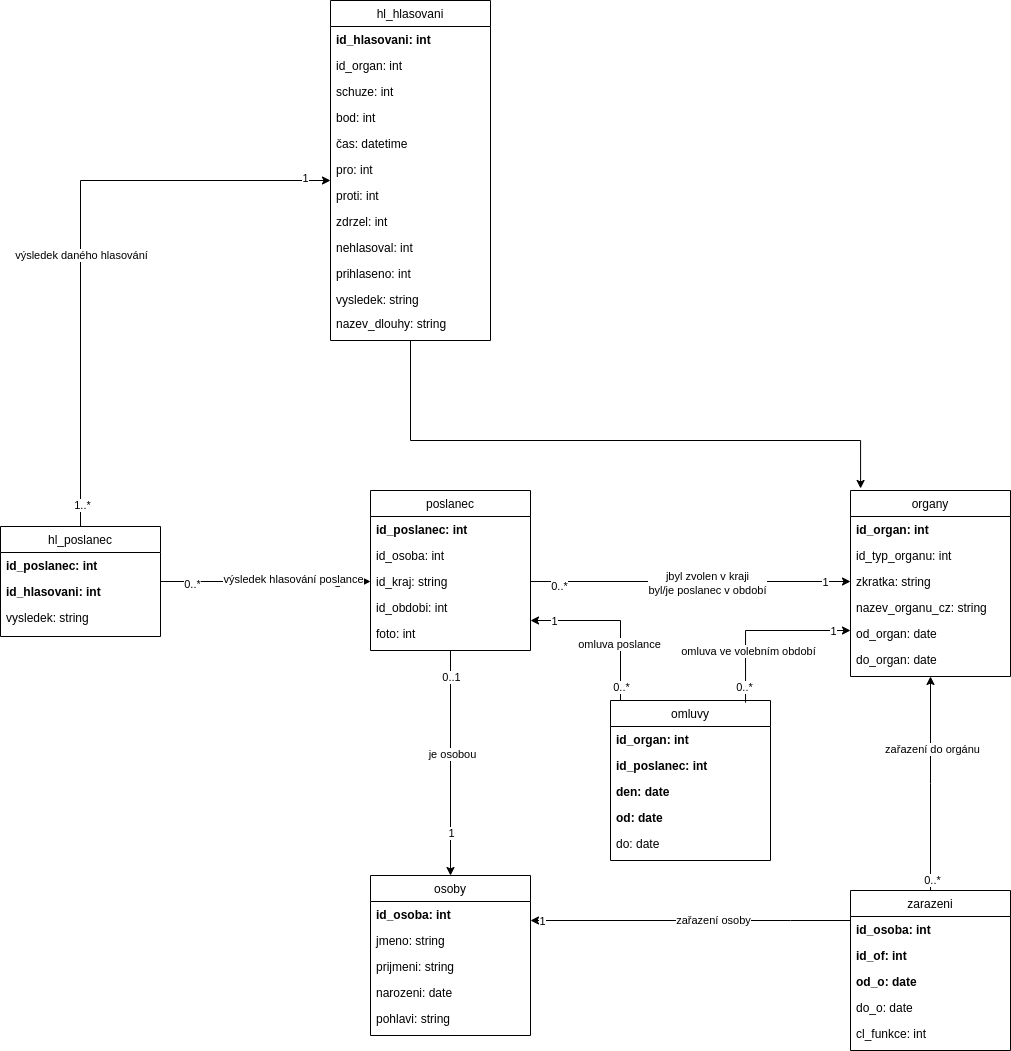
\includegraphics[width=\linewidth]{source_data_diagram}
	\caption{Diagram zdrojových dat}
	\label{fig:class-diagram}
\end{figure}

\begin{figure}[h]
	\begin{minipage}{0.5\textwidth}
		\centering
		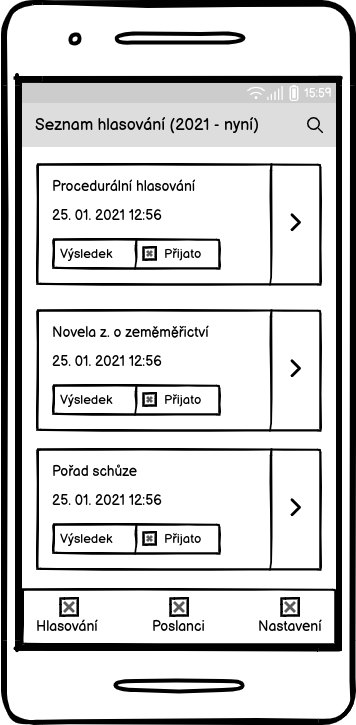
\includegraphics[scale = 0.5]{vote_list.png}
		\caption{Seznam hlasování}
		\label{fig:vote_list}
	\end{minipage}%
	\begin{minipage}{0.5\textwidth}
		\centering
		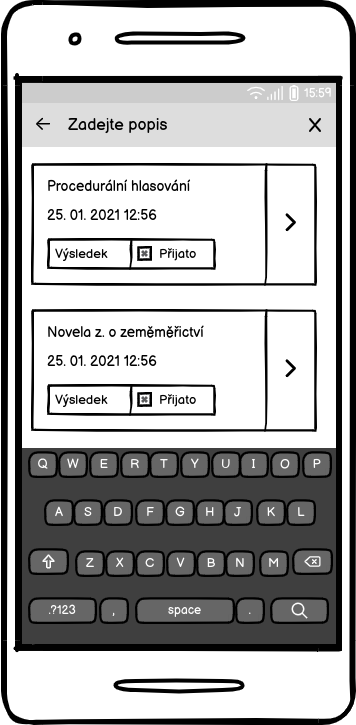
\includegraphics[scale = 0.5]{vote_list_search.png}
		\caption{Vyhledávání v seznamu hlasování}
		\label{fig:vote_list_search}
	\end{minipage}
	\caption{Obrazovka pro seznam hlasování}
\end{figure}

\begin{figure}[h]
	\begin{minipage}{0.5\textwidth}
		\centering
		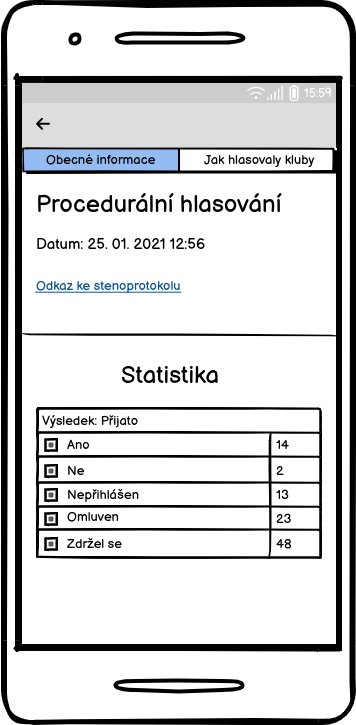
\includegraphics[scale = 0.4]{vote_details_general.png}
		\caption{Detail hlasování}
		\label{fig:vote_details_general}
	\end{minipage}%
	\begin{minipage}{0.5\textwidth}
		\centering
		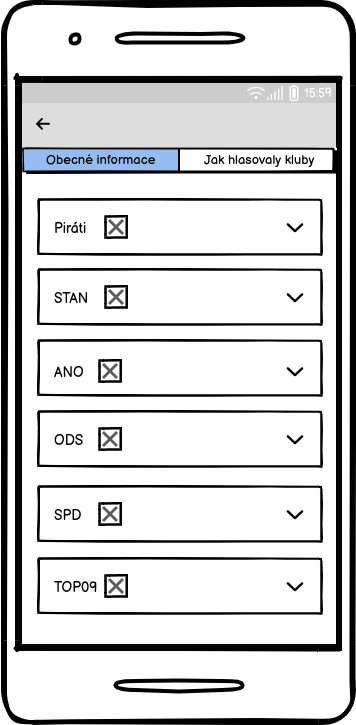
\includegraphics[scale = 0.4]{vote_details_party_votes.png}
		\caption{Jak hlasovaly kluby}
		\label{fig:vote_details_party_votes}
	\end{minipage}
	\begin{minipage}{0.5\textwidth}
	\centering
	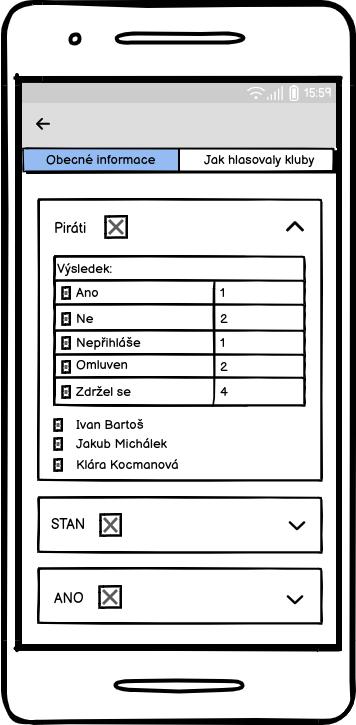
\includegraphics[scale = 0.4]{vote_details_party_votes_expanded.png}
	\caption{Jak hlasovaly kluby}
	\label{fig:vote_details_party_votes_expanded}
\end{minipage}
	\caption{Obrazovky pro detail hlasování}
\end{figure}

\begin{figure}[h]
	\begin{minipage}{0.5\textwidth}
		\centering
		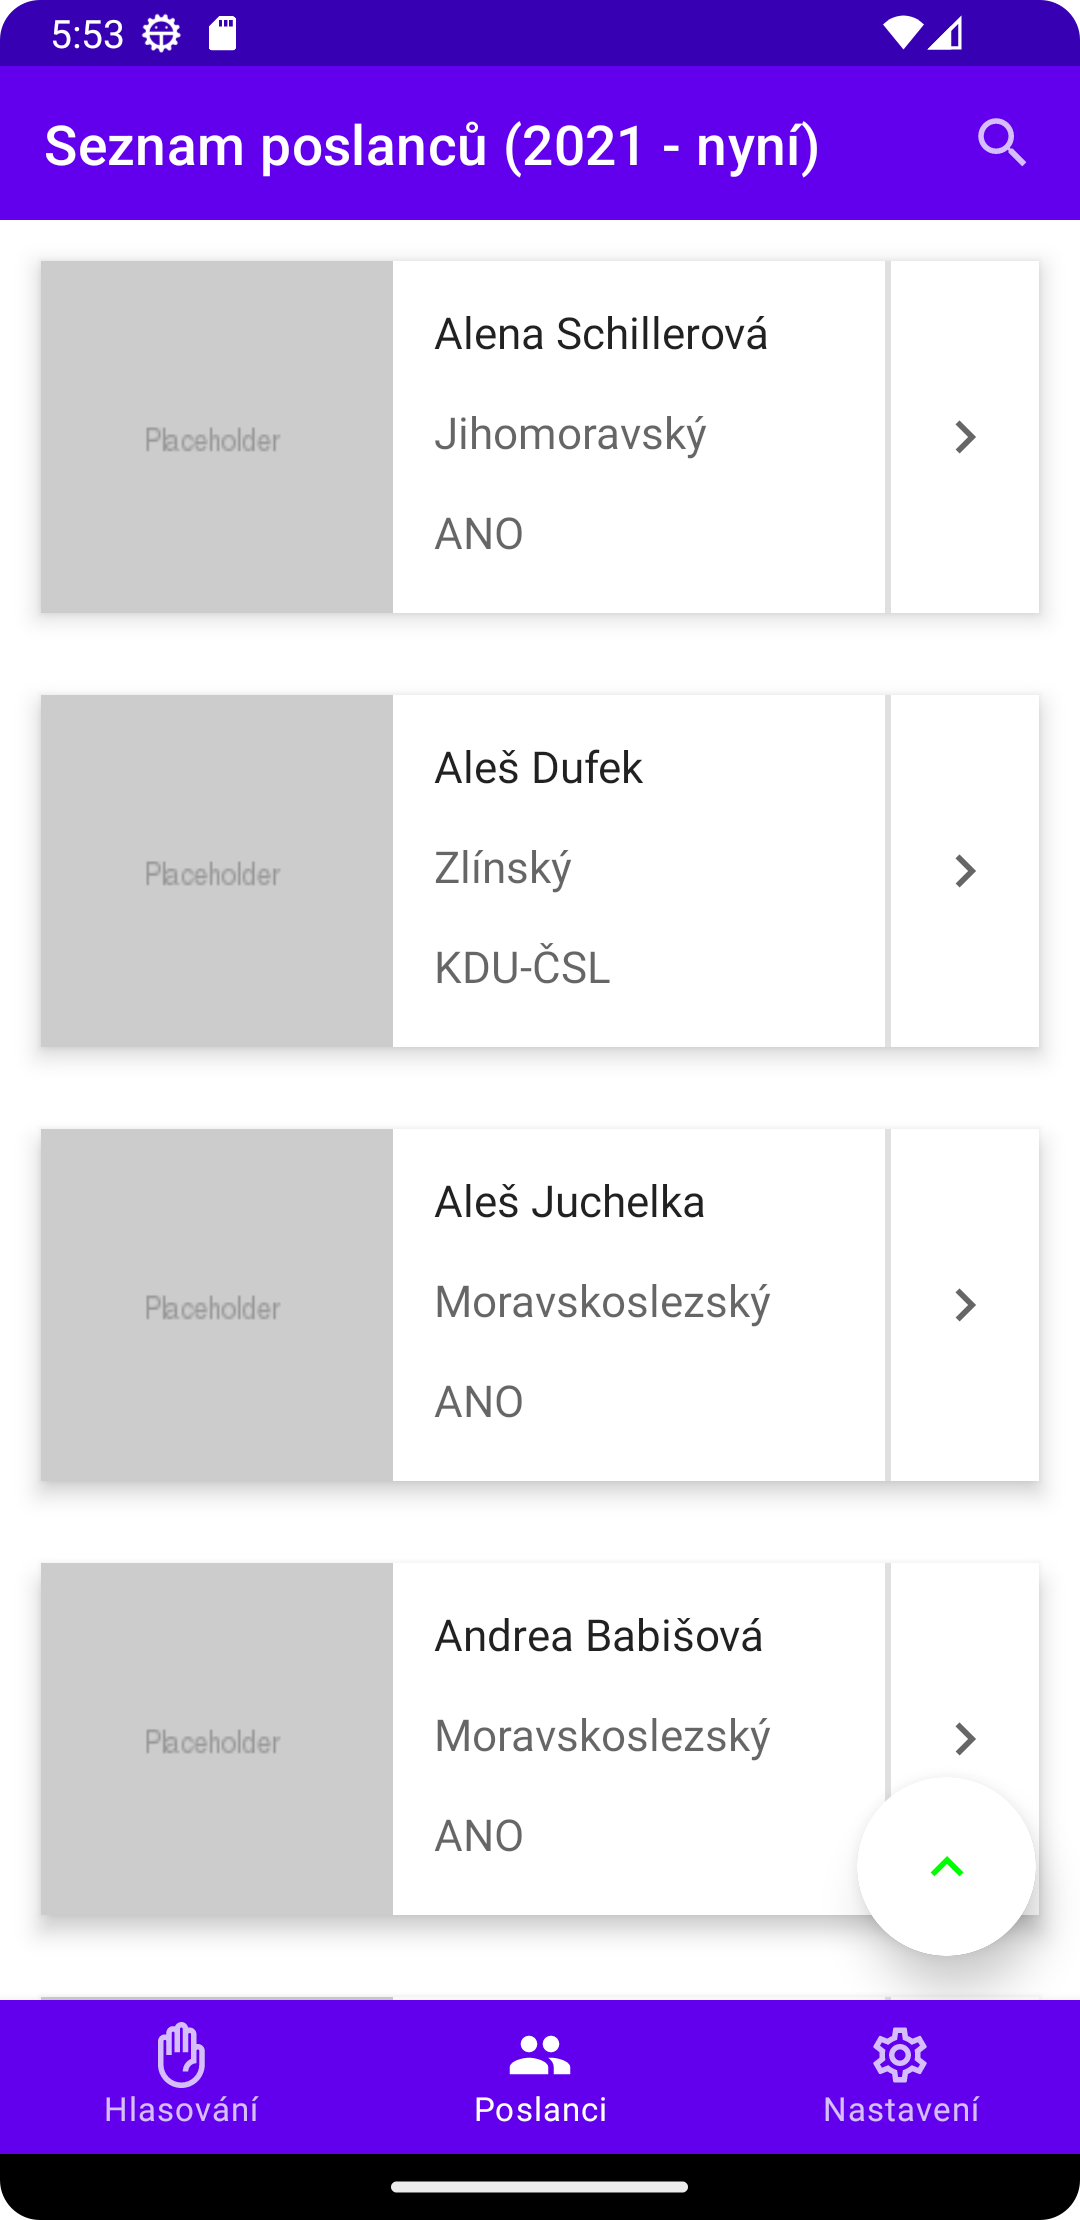
\includegraphics[scale = 0.5]{member_list.png}
		\caption{Seznam poslanců}
		\label{fig:member_list}
	\end{minipage}%
	\begin{minipage}{0.5\textwidth}
		\centering
		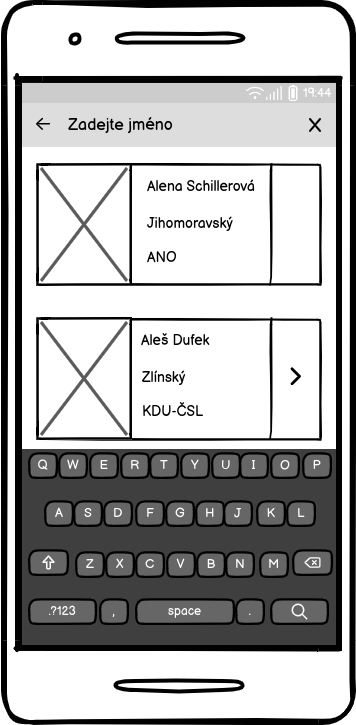
\includegraphics[scale = 0.5]{member_list_search.png}
		\caption{Vyhledávání v seznamu poslanců}
		\label{fig:member_list_search}
	\end{minipage}
	\caption{Obrazovka pro seznam poslanců}
\end{figure}

\begin{figure}[h]
	\begin{minipage}{0.5\textwidth}
		\centering
		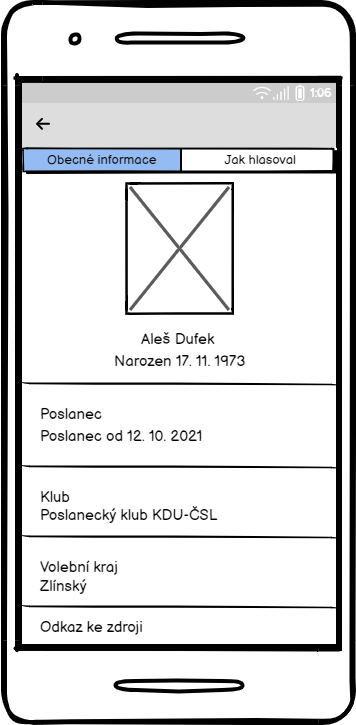
\includegraphics[scale = 0.5]{member_details_general.png}
		\caption{Detail poslance}
		\label{fig:member_details_general}
	\end{minipage}%
	\begin{minipage}{0.5\textwidth}
		\centering
		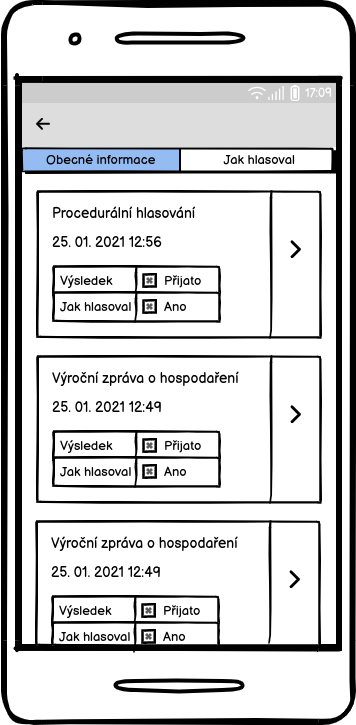
\includegraphics[scale = 0.5]{member_details_votes.png}
		\caption{Jak hlasoval/a poslanec/kyně}
		\label{fig:member_details_votes}
	\end{minipage}
	\caption{Obrazovky pro detail poslance}
\end{figure}

\begin{figure}[h]
	\begin{minipage}{0.5\textwidth}
		\centering
		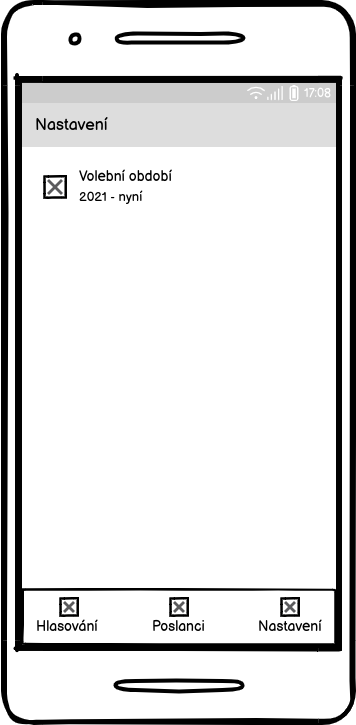
\includegraphics[scale = 0.5]{settings.png}
		\caption{Seznam nastavení}
		\label{fig:settings}
	\end{minipage}%
	\begin{minipage}{0.5\textwidth}
		\centering
		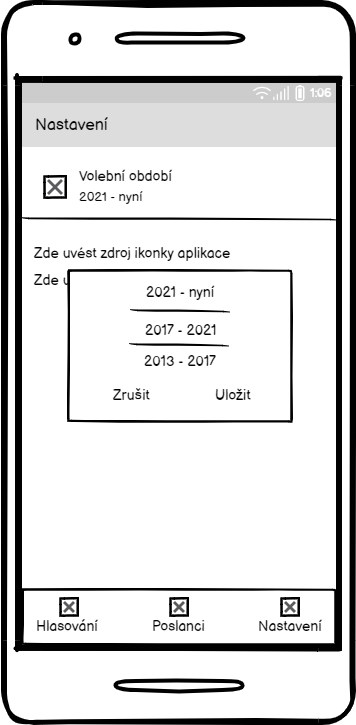
\includegraphics[scale = 0.5]{settings_opened.png}
		\caption{Nastavení volebního období}
		\label{fig:settings_opened}
	\end{minipage}
	\caption{Obrazovka pro nastavení}
\end{figure}

\begin{lstlisting}[caption={Tělo odpovědi pro dotaz \lstinline{GET /api/app}.}, label={fig:app}, language=json,firstnumber=1,tabsize=2]
{
	"election_years": [
	2021,
	2017,
	2013,
	2010,
	2006,
	2002,
	1998,
	1996,
	1992
	]
}
\end{lstlisting}

\begin{lstlisting}[caption={Tělo odpovědi pro dotaz \lstinline{GET /api/vote}}, label={fig:vote}, language=json,firstnumber=1,tabsize=2]
[
	{
		"id": 1,
		"date_time": "16. 12. 2022 13:29",
		"description": "Hlasovani 1",
		"result": "A"
	},
	{
		"id": 2,
		"date_time": "16. 12. 2022 13:26",
		"description": "Hlasovani 2",
		"result": "A"
	},
]
\end{lstlisting}

\begin{lstlisting}[caption={Tělo odpovědi pro dotaz \lstinline{GET /api/vote{id}}}, label={fig:vote-1}, language=json,firstnumber=1,tabsize=2]
{
	"id": 1,
	"date_time": "16. 12. 2022 13:29",
	"description": "Hlasovani 1,
	"result": "A",
	"steno_protocol_url": "http://www.psp.cz/eknih/2021ps/stenprot/048schuz/s048109.htm#h76",
	"yes_count": 100,
	"no_count": 0,
	"logged_off_count": 64,
	"excused_count": 0,
	"refrained_count": 36,
	"election_year": 0
}
\end{lstlisting}

\begin{lstlisting}[caption={Tělo odpovědi pro dotaz \lstinline{GET /api/party/vote/1}}, label={fig:party-vote-1}, language=json,firstnumber=1,tabsize=2]
[
	{
		"party_name": "Nazev klubu",
		"logo_url": "https://www.psp.cz/pics/klub/l-cps.jpg",
		"vote_id": 1,
		"party_results": {
			"yes_count": 2,
			"no_count": 0,
			"logged_off_count": 1,
			"excused_count": 0,
			"refrained_count": 0
		},
		"member_results": [
			{
				"member_name": "Poslanec 1",
				"vote_result": "@"
			},
			{
				"member_name": "Poslanec 2",
				"vote_result": "C"
			},
			{
				"member_name": "Poslanec 3",
				"vote_result": "A"
			},
			{
				"member_name": "Poslanec 4",
				"vote_result": "A"
			}
		]
	}
]
\end{lstlisting}

\begin{lstlisting}[caption={Tělo odpovědi pro dotaz ¨}, label={fig:member}, language=json,firstnumber=1,tabsize=2]
[
	{
		"id": 1,
		"name": "Poslanec 1",
		"party": "ANO",
		"photo_url": "https://www.psp.cz/eknih/cdrom/2021ps/eknih/2021ps/poslanci/i6474.jpg",
		"election_region": "Volebni kraj 1",
		"election_year": 2021
	},
	{
		"id": 2,
		"name": "Poslanec 2",
		"party": "ODS",
		"photo_url": "https://www.psp.cz/eknih/cdrom/2021ps/eknih/2021ps/poslanci/i6804.jpg",
		"election_region": "Volebni kraj 2",
		"election_year": 2021
	},
]
\end{lstlisting}

\begin{lstlisting}[caption={Tělo odpovědi pro dotaz \lstinline{GET /api/member/1}}, label={fig:member-1}, language=json,firstnumber=1,tabsize=2]
{
	"id": 1,
	"name": "Poslanec 1",
	"gender": "M",
	"party": "Poslanecky klub",
	"member_from": "12. 10. 2021",
	"member_to": null,
	"date_of_birth": "25. 09. 1970",
	"election_region": "Volebni kraj 1",
	"photo_url": "https://www.psp.cz/eknih/cdrom/2021ps/eknih/2021ps/poslanci/i6474.jpg",
	"election_year": 2021
}
\end{lstlisting}

\begin{lstlisting}[caption={Tělo odpovědi pro dotaz \lstinline{GET /api/member/1/vote}}, label={fig:member-vote-1}, language=json,firstnumber=1,tabsize=2]
[
	{
		"vote": {
			"id": 1,
			"date_time": "16. 12. 2022 13:29",
			"description": "Hlasovani 1",
			"result": "A"
		},
		"how_member_voted": "@"
	},
	{
		"vote": {
			"id": 2,
			"date_time": "16. 12. 2022 13:26",
			"description": "Hlasovani 2",
			"result": "A"
		},
		"how_member_voted": "@"
	}
]
\end{lstlisting}

\begin{table}[!h]\centering
	\caption[Struktura agency]{Struktura agency}\label{table:agency}
	\begin{tabular}{|l|l|p{6cm}|}\hline
		Název	& Typ	& Popis	\tabularnewline \hline \hline
		\texttt{id}		& \texttt{int}	& identifikátor orgánu		\tabularnewline \hline
		\texttt{abbreviation}		& \texttt{varchar(255)}	& zkratka názvu orgánu		\tabularnewline \hline
		\texttt{end\textunderscore date}		& \texttt{date(255)}	& datum zániku orgánu		\tabularnewline \hline
		\texttt{name}		& \texttt{varchar(255)}	& název orgánu		\tabularnewline \hline
		\texttt{start\textunderscore date}		& \texttt{date}	& datum založení orgánu		\tabularnewline \hline
		\texttt{type\textunderscore id}		& \texttt{int}	& identifikátor typu orgánu 		\tabularnewline \hline
	\end{tabular}
\end{table}

\begin{table}[!h]\centering
	\caption[Struktura agency\textunderscore type]{Struktura agency\textunderscore type}\label{table:agency_type}
	\begin{tabular}{|l|l|p{6cm}|}\hline
		Název	& Typ	& Popis	\tabularnewline \hline \hline
		\texttt{id}		& \texttt{int}	& identifikátor typu orgánu		\tabularnewline \hline
		\texttt{name}		& \texttt{varchar(512)}	& název typu orgánu \tabularnewline \hline
		\texttt{superior\textunderscore agency\textunderscore type\textunderscore id}		& \texttt{int}	& identifikátor nadřazeného typu orgánu \tabularnewline \hline
	\end{tabular}
\end{table}

\begin{table}[!h]\centering
	\caption[Struktura excuse]{Struktura excuse}\label{table:excuse}
	\begin{tabular}{|l|l|p{6cm}|}\hline
		Název	& Typ	& Popis	\tabularnewline \hline \hline
		\texttt{member\textunderscore id}		& \texttt{int}	& identifikátor poslance, který je omluven		\tabularnewline \hline
		\texttt{date} & \texttt{date}	& datum, kdy je poslanec omluven \tabularnewline \hline
		\texttt{start\textunderscore time}		& \texttt{time}	& čas, od kterého byl poslanec omluven \tabularnewline \hline
		\texttt{end\textunderscore time}		& \texttt{time}	& čas, do kterého byl poslanec omluven \tabularnewline \hline
		\texttt{election\textunderscore year}		& \texttt{int}	& první rok volebního období \tabularnewline \hline
	\end{tabular}
\end{table}

\begin{table}[!h]\centering
	\caption[Struktura member]{Struktura member}\label{table:member}
	\begin{tabular}{|l|l|p{6cm}|}\hline
		Název	& Typ	& Popis	\tabularnewline \hline \hline
		\texttt{id}		& \texttt{int}	& identifikátor poslance, který je omluven		\tabularnewline \hline
		\texttt{date\textunderscore of\textunderscore birth} & \texttt{date}	& datum narození \tabularnewline \hline
		\texttt{election\textunderscore region}		& \texttt{varchar(255)}	& volební kraj \tabularnewline \hline
		\texttt{election\textunderscore year}		& \texttt{int}	& první rok volebního období \tabularnewline \hline
		\texttt{gender}		& \texttt{varchar(255)}	& pohlaví \tabularnewline \hline
		\texttt{member\textunderscore from} & \texttt{date} & datum začátku členství \tabularnewline \hline
		\texttt{member\textunderscore to} & \texttt{date} & datum konce členství \tabularnewline \hline
		\texttt{name} & \texttt{varchar(255)} & jméno \tabularnewline \hline
		\texttt{person\textunderscore id} & \texttt{int} & identifikátor osoby \tabularnewline \hline
		\texttt{photo\textunderscore url} & \texttt{varchar(255)} & URL profilové fotky \tabularnewline \hline
		\texttt{party\textunderscore election\textunderscore year} & \texttt{int} & první rok volebního období \tabularnewline \hline
		\texttt{party\textunderscore party\textunderscore id} & \texttt{int} & identifikíátor poslaneckého klubu, jehož je členem \tabularnewline \hline
	\end{tabular}
\end{table}

\begin{table}[!h]\centering
	\caption[Struktura member\textunderscore vote]{Struktura member\textunderscore vote}\label{table:membe_vote}
	\begin{tabular}{|l|l|p{6cm}|}\hline
		Název	& Typ	& Popis	\tabularnewline \hline \hline
		\texttt{result}		& \texttt{varchar(255)}	& jak hlasoval poslanec\tabularnewline \hline
		\texttt{member\textunderscore id}		& \texttt{int}	& jak identifikátor poslance\tabularnewline \hline
		\texttt{vote\textunderscore id}		& \texttt{int}	& identifikátor hlasování\tabularnewline \hline
	\end{tabular}
\end{table}

\begin{table}[!h]\centering
	\caption[Struktura membership]{Struktura membership}\label{table:membership}
	\begin{tabular}{|l|l|p{6cm}|}\hline
		Název	& Typ	& Popis	\tabularnewline \hline \hline
		\texttt{end\textunderscore date}		& \texttt{datetime}	& datum a čas konce zařazení\tabularnewline \hline
		\texttt{agency\textunderscore id}		& \texttt{int}	& identifikátor orgánu\tabularnewline \hline
		\texttt{person\textunderscore id}		& \texttt{int}	& identifikátor osoby \tabularnewline \hline
		\texttt{start\textunderscore date}		& \texttt{datetime}	& datum a čas začátku zařazení \tabularnewline \hline
	\end{tabular}
\end{table}

\begin{table}[!h]\centering
	\caption[Struktura party]{Struktura party}\label{table:party}
	\begin{tabular}{|l|l|p{6cm}|}\hline
		Název	& Typ	& Popis	\tabularnewline \hline \hline
		\texttt{abbreviation} & \texttt{varchar(255)} & zkratka pro název klubu\tabularnewline \hline
		\texttt{name} & \texttt{varchar(255)}	& název klubu\tabularnewline \hline
		\texttt{election\textunderscore year}		& \texttt{int}	& první rok volebního období \tabularnewline \hline
		\texttt{party\textunderscore id}		& \texttt{int}	& identifikátor klubu \tabularnewline \hline
	\end{tabular}
\end{table}

\begin{table}[!h]\centering
	\caption[Struktura vote]{Struktura vote}\label{table:vote}
	\begin{tabular}{|l|l|p{6cm}|}\hline
		Název	& Typ	& Popis	\tabularnewline \hline \hline
		\texttt{date\textunderscore time} & \texttt{datetime} & datum a čas hlasování\tabularnewline \hline
		\texttt{description} & \texttt{varchar(255)}	& popis hlasování\tabularnewline \hline
		\texttt{election\textunderscore year}		& \texttt{int}	& první rok volebního období \tabularnewline \hline
		\texttt{excused\textunderscore count}		& \texttt{int}	& počet omluvených \tabularnewline \hline
		\texttt{logged\textunderscore off\textunderscore count}		& \texttt{int}	& počet nepřihlášených \tabularnewline \hline
		\texttt{meeting\textunderscore number}		& \texttt{int}	& bod hlasování \tabularnewline \hline
		\texttt{no\textunderscore count}		& \texttt{int}	& počet hlasování proti \tabularnewline \hline
		\texttt{refrained\textunderscore count}		& \texttt{int}	& počet zdržených \tabularnewline \hline
		\texttt{result}		& \texttt{varchar(255)}	& výsledek hlasování \tabularnewline \hline
		\texttt{steno\textunderscore protocol\textunderscore url}		& \texttt{varchar(255)}	& stenoprotokol \tabularnewline \hline
		\texttt{yes\textunderscore count}		& \texttt{int}	& počet hlasování pro \tabularnewline \hline
		\texttt{number}		& \texttt{int}	& číslo hlasování \tabularnewline \hline
		\texttt{id}		& \texttt{int}	& identifikátor hlasování \tabularnewline \hline
	\end{tabular}
\end{table}

\begin{figure}
	\centering
	\begin{minipage}{\textwidth}
		\dirtree{%
			.1 app.
			.2 src.
			.3 main.
			.4 java.
			.5 com.lukas\_dang.psp\_fe.
			.6 app.
			.7 navigation\DTcomment{Zdrojové kódy pro navigaci mezi obrazovkami}.
			.7 ui.
			.8 theme\DTcomment{Barvy, typografie, barevné režimy, tvary}.
			.8 PspApp.kt\DTcomment{Hlavní komponenta aplikace}.
			.8 PspAppState.kt\DTcomment{Stav aplikace}.
			.7 MainActivity\DTcomment{Hlavní aktivita}.
			.7 PspApplication\DTcomment{Třída reprezentující aplikaci}.
			.6 core\DTcomment{Stav aplikace}.
			.6 feature.
			.4 proto.
			.5 user\_prefs.proto.
			.4 res.
			.5 drawable.
			.5 values.
			.6 strings.xml.
			.4 AndroidManifest.xml.
			.3 test\DTcomment{Unit testy}.
			.3 androidTest\DTcomment{Instrumentované testy}.
			.2 build.gradle.
			.1 build.gradle.
		}
	\end{minipage}
	\caption{Adresářová struktura mobilní aplikace}
	\label{fig:dir_struct}
\end{figure}
